\documentclass[10pt,twocolumn,letterpaper]{article}

\usepackage{tikz}
\usetikzlibrary{shapes.geometric, arrows.meta, positioning}
\usepackage[article]{cvpr}

% Include other packages here, before hyperref.
\usepackage{graphicx}
\usepackage{amsmath}
\usepackage{amssymb}
\usepackage{booktabs}
\usepackage{ctable}
\usepackage{multirow}
\usepackage{array}
\usepackage{colortbl}
\usepackage[ruled,vlined,linesnumbered]{algorithm2e}

\definecolor{cvprblue}{rgb}{0.21,0.49,0.74}
\usepackage[pagebackref,breaklinks,colorlinks,citecolor=cvprblue]{hyperref}

\def\paperID{}
\def\confName{CVPR}
\def\confYear{}

\begin{document}
	
	\title{Iterative Neural Architecture Search via LLM-Driven Code Generation with Historical Feedback Memory}
	
	\author{Name Surname{\thanks{Corresponding author: email@uni-wuerzburg.de}}, \space\space\space Name Surname,\space\space\space Name Surname,\space\space\space Dmitry Ignatov,\space\space\space Radu Timofte\\
		\small{Computer Vision Lab, CAIDAS \& IFI, University of W\"urzburg, Germany}}
	\maketitle
	
	
	%%%%%%%%% ABSTRACT
	\begin{abstract}
		Neural Architecture Search (NAS) automates network design but typically demands substantial computational resources. We propose a closed-loop pipeline that leverages a small (4-billion-parameter) large language model (LLM) to iteratively generate, evaluate, and refine convolutional neural network architectures for image classification. Central to our approach is a \emph{historical feedback memory} mechanism inspired by Markov chains: a sliding window of the most recent improvement attempts is fed back to the LLM, enabling it to learn from past successes and failures without additional training. Using one-epoch proxy accuracy on CIFAR-10 as a fast architecture ranking signal, our pipeline improves generated architectures from 22.2\% to 59.2\% top-1 accuracy over 100 successful evaluations (Spearman $\rho = 0.70$, $p < 10^{-15}$), representing a $2.7\times$ improvement over single-shot generation. These results demonstrate that even small LLMs can serve as effective architecture designers when equipped with iterative feedback and historical memory, offering a lightweight and accessible paradigm for LLM-driven NAS.
	\end{abstract}
	
	%%%%%%%%% BODY TEXT
	\section{Introduction}
	\label{sec:intro}
	
	Neural Architecture Search (NAS) has emerged as a powerful paradigm for automating the design of deep neural networks, achieving competitive or superior performance to hand-crafted architectures across diverse tasks~\cite{Zoph2017,Real2019,Liu2019DARTS}. However, conventional NAS methods---whether based on reinforcement learning~\cite{Zoph2017}, evolutionary algorithms~\cite{Real2019}, or differentiable relaxations~\cite{Liu2019DARTS}---remain computationally expensive, often requiring hundreds or thousands of GPU hours to search a single architecture. This cost has motivated training-free approaches that use proxy metrics to rank architectures without full training~\cite{Mellor2021,Li2024ZeroShot}, yet these methods still operate within predefined, discrete search spaces.
	
	Recent advances in large language models (LLMs) have opened a fundamentally different avenue: using LLMs as architecture generators that produce executable neural network code directly~\cite{ABrain.NNGPT,ABrain.Architect,ABrain.Prompt}. Unlike traditional NAS, LLM-based approaches operate in the space of \emph{programs} rather than fixed cell-based encodings, enabling more flexible and expressive architecture design. Prior work within the NNGPT framework~\cite{ABrain.NNGPT} and related efforts~\cite{ABrain.NN-Captioning_2025,ABrain.NNGPT-Fractal,ABrain.CV_Channel} have demonstrated that LLMs can generate functional vision models, but predominantly through single-shot or few-shot generation without iterative self-improvement.
	
	A critical limitation of single-shot LLM generation is that it treats architecture design as a one-pass prediction, discarding the evaluation signal entirely. In contrast, human engineers iterate: they build, test, analyze failures, and refine their designs based on accumulated experience. This observation motivates our central question: \emph{Can a small LLM iteratively improve neural network architectures by learning from a structured history of its own attempts?}
	
	We propose a closed-loop pipeline comprising three components: (1)~a \textbf{Code Generator} that prompts a 4-billion-parameter LLM to produce PyTorch model implementations, (2)~an \textbf{Evaluator} that trains each generated model for a single epoch on CIFAR-10 as a fast proxy for architecture quality, and (3)~a \textbf{Prompt Improver} that analyzes evaluation results alongside a sliding window of recent iteration history---a mechanism we term \emph{historical feedback memory}---to produce targeted improvement suggestions for the next iteration. This design draws on the Markov property: the improvement decision at each step depends on the current best architecture and a bounded window of recent transitions, rather than the full trajectory.
	
	Our main contributions are:
	\begin{itemize}
		\item A closed-loop, iterative NAS pipeline driven by a small (4B-parameter) LLM that progressively discovers better architectures through code generation, evaluation, and prompt refinement.
		\item A \emph{historical feedback memory} mechanism that maintains a sliding window of past improvement attempts, enabling the LLM to avoid repeating failed strategies and build on successful ones.
		\item An empirical demonstration that this pipeline improves architecture quality from 22.2\% to 59.2\% one-epoch proxy accuracy on CIFAR-10 over 100 evaluations, with a strong positive trend (Spearman $\rho = 0.70$, $p < 10^{-15}$).
	\end{itemize}
	
	
	\section{Related Work}
	\label{sec:Related}
	
	\paragraph{Neural Architecture Search.}
	NAS methods aim to automate the design of neural network architectures. Early approaches employed reinforcement learning~\cite{Zoph2017} and evolutionary algorithms~\cite{Real2019} to explore architecture search spaces, but required thousands of GPU hours per search. Parameter-sharing methods such as ENAS~\cite{Pham2018} and differentiable approaches like DARTS~\cite{Liu2019DARTS} substantially reduced search cost by amortizing evaluation across architectures. More recently, \emph{zero-shot} or \emph{training-free} NAS methods~\cite{Mellor2021,Li2024ZeroShot} bypass training entirely by scoring architectures at initialization using proxy metrics such as activation overlap~\cite{Mellor2021} or gradient-based indicators. While effective within their respective search spaces, these methods remain constrained to predefined, discrete architecture parameterizations (e.g., cell-based structures) and cannot generate truly novel architectural patterns.
	
	\paragraph{LLMs for Code Generation and AutoML.}
	Large language models have demonstrated strong capabilities in code generation~\cite{Chen2021Codex}, and their application to machine learning automation is an active research area. The NNGPT framework~\cite{ABrain.NNGPT} pioneered the use of LLMs as neural network generators, showing that language models can produce functional vision models from textual prompts. Subsequent work explored fractal-inspired architectures~\cite{ABrain.NNGPT-Fractal}, few-shot prompting strategies~\cite{ABrain.Prompt}, novel architecture creativity~\cite{ABrain.Architect}, and non-standard channel priors~\cite{ABrain.CV_Channel}. LLMs have also been applied to hyperparameter optimization~\cite{ABrain.HPGPT}, data transformation design~\cite{ABrain.Transform}, and collaborative vision-language pipelines~\cite{Rupani2025llm,Gado2025llm,ABrain.NN-RAG}. These efforts are supported by curated datasets of neural network architectures~\cite{ABrain.NN-Dataset,ABrain.LEMUR2} and deployment pipelines~\cite{ABrain.NN-Lite}. However, most existing approaches treat LLM-based architecture generation as a single-step process, without leveraging iterative refinement from evaluation feedback. Our work extends this line by introducing a closed-loop pipeline with historical memory that enables progressive architecture improvement.
	
	
	\section{Methodology}
	\label{sec:Methodology}
	
	Inspired by recent advancements in the application of LLMs across various domains~\cite{ABrain.HPGPT,Gado2025llm,Rupani2025llm,ABrain.NN-RAG} and prior architectural synthesis experiments within the NNGPT framework~\cite{ABrain.HPGPT,ABrain.NN-Captioning_2025,ABrain.Prompt,ABrain.NNGPT-Fractal,ABrain.Transform,ABrain.Architect,ABrain.CV_Channel}, and leveraging the existing LEMUR dataset of a broad range of high-capacity and edge-optimized models~\cite{ABrain.NN-Dataset,ABrain.LEMUR2,ABrain.NN-Lite}, we developed an iterative NAS pipeline based on the NNGPT framework~\cite{ABrain.NNGPT}. The pipeline consists of three core modules operating in a closed loop, as illustrated in Figure~\ref{fig:pipeline}.
	
	\subsection{Pipeline Overview}
	
	At each iteration $t$, the pipeline executes the following cycle: (1)~the Code Generator produces a candidate architecture $\mathcal{A}_t$ as executable PyTorch code; (2)~the generated code is validated and, if structurally correct, trained and evaluated by the Evaluator to obtain a proxy accuracy $a_t$; (3)~the Prompt Improver analyzes the result in the context of the current best architecture and recent iteration history, producing improvement suggestions $s_t$ for the next iteration. The best-performing architecture $\mathcal{A}^* = \arg\max_{i \leq t} a_i$ is maintained as the reference implementation throughout the search.
	
	\subsection{Code Generator}
	
	The Code Generator uses a pre-trained LLM (Qwen3-4B-Instruct, a 4-billion-parameter instruction-tuned model) to produce a complete PyTorch model class implementing \texttt{nn.Module}. The LLM receives a fixed prompt template comprising: (i)~a role description positioning the model as a ``visionary deep learning architect,'' (ii)~the task specification (CIFAR-10 image classification without pre-trained weights), (iii)~the current best implementation $\mathcal{A}^*$ as reference code, and (iv)~the improvement suggestions $s_{t-1}$ from the previous iteration. The generated code must define a \texttt{Net(nn.Module)} class with standard \texttt{\_\_init\_\_} and \texttt{forward} methods. Generation uses temperature $\tau = 0.7$ and nucleus sampling ($p = 0.9$) to balance architectural diversity with code coherence.
	
	\subsection{Evaluator}
	
	Generated code undergoes a two-stage evaluation process.
	
	\textbf{Quick validation.} The model is instantiated and a forward pass is performed with a dummy input tensor of shape $2 \times 3 \times 32 \times 32$. The output shape is verified to match $B \times 10$ (for batch size $B$ and 10 CIFAR-10 classes). Models failing this check are discarded with an error message forwarded to the Prompt Improver.
	
	\textbf{Proxy training.} Models passing validation are trained for \textbf{one epoch} on CIFAR-10 using SGD (momentum $0.9$, weight decay $5 \times 10^{-4}$), an initial learning rate of $0.01$ with cosine annealing, and a batch size of $128$. Standard data augmentation is applied: random crop with 4-pixel padding and random horizontal flip. Top-1 test accuracy on the 10,000-image test set serves as the proxy metric. Training is executed in an isolated subprocess with a 30-minute timeout. One-epoch accuracy provides a fast, informative signal for ranking architectures~\cite{Mellor2021}, enabling rapid iteration without the cost of full convergence training.
	
	\subsection{Prompt Improver with Historical Feedback Memory}
	\label{sec:history}
	
	The Prompt Improver is the central component enabling iterative learning. After each evaluation, it receives three inputs: (1)~the best code $\mathcal{A}^*$ and its accuracy $a^*$, (2)~the current iteration's code $\mathcal{A}_t$ and its evaluation outcome (accuracy value or error message), and (3)~a \emph{historical feedback memory} $\mathcal{H}_t$ containing the last $K{=}5$ improvement attempts.
	
	Each history entry $h_i \in \mathcal{H}_t$ is a triple recording: the identified problem, the suggested improvement, and the resulting outcome (accuracy achieved or error encountered). This sliding-window design draws on the Markov property: the improvement decision at step $t$ depends on the current state (best architecture plus recent history window) rather than the complete trajectory. The bounded window prevents context overflow while providing sufficient signal for the LLM to identify recurring failure patterns.
	
	The Prompt Improver produces a structured response containing: (a)~a \textbf{reason} diagnosing the current result, (b)~an \textbf{inspiration} drawing on cross-disciplinary insights, and (c)~concrete \textbf{improvement suggestions} for the next iteration. These suggestions, together with the best code, form the input to the Code Generator in the subsequent iteration, closing the feedback loop.
	
	The overall procedure is summarized in Algorithm~\ref{alg:pipeline}.
	
	\begin{algorithm}[t]
		\caption{Iterative LLM-Driven NAS Pipeline}
		\label{alg:pipeline}
		\KwIn{LLM $\mathcal{L}$, max iterations $T$, history window $K$}
		$\mathcal{A}^* \leftarrow \emptyset$; $a^* \leftarrow 0$; $\mathcal{H} \leftarrow \emptyset$; $s_0 \leftarrow \emptyset$\;
		\For{$t \leftarrow 1$ \KwTo $T$}{
			$\mathcal{A}_t \leftarrow \text{Generate}(\mathcal{L}, \mathcal{A}^*, s_{t-1})$\;
			\eIf{$\text{Validate}(\mathcal{A}_t)$ succeeds}{
				$a_t \leftarrow \text{TrainAndEvaluate}(\mathcal{A}_t)$\;
			}{
				$a_t \leftarrow$ error message\;
			}
			\If{$a_t > a^*$}{
				$\mathcal{A}^* \leftarrow \mathcal{A}_t$; $a^* \leftarrow a_t$\;
			}
			Append $(s_{t-1}, a_t)$ to $\mathcal{H}$; keep last $K$ entries\;
			$s_t \leftarrow \text{Improve}(\mathcal{L}, \mathcal{A}^*, \mathcal{A}_t, a_t, \mathcal{H})$\;
		}
		\Return $\mathcal{A}^*$, $a^*$
	\end{algorithm}
	
	\begin{figure}[t]
		\centering
		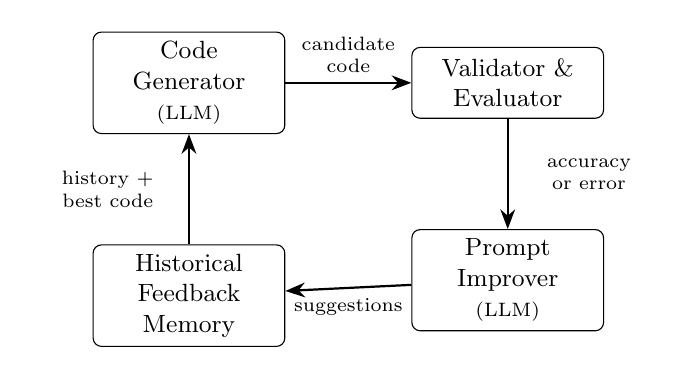
\begin{tikzpicture}[
			node distance=1.4cm and 1.6cm,
			block/.style={rectangle, draw, rounded corners=3pt, text width=2.2cm, text centered, minimum height=0.9cm, font=\small},
			arrow/.style={-{Stealth[length=2.5mm]}, thick},
			label/.style={font=\scriptsize, text width=1.8cm, align=center}
			]
			\node[block] (gen) {Code\\Generator\\{\scriptsize(LLM)}};
			\node[block, right=of gen] (eval) {Validator \&\\Evaluator};
			\node[block, below=of eval] (imp) {Prompt\\Improver\\{\scriptsize(LLM)}};
			\node[block, below=of gen] (hist) {Historical\\Feedback\\Memory};
			
			\draw[arrow] (gen) -- node[above, label] {candidate\\code} (eval);
			\draw[arrow] (eval) -- node[right, label] {accuracy\\or error} (imp);
			\draw[arrow] (imp) -- node[below, label] {suggestions} (hist);
			\draw[arrow] (hist) -- node[left, label] {history +\\best code} (gen);
		\end{tikzpicture}
		\caption{Overview of the iterative NAS pipeline. The Code Generator produces candidate architectures as executable PyTorch code. The Evaluator validates and trains them using one-epoch proxy evaluation. The Prompt Improver analyzes results with historical feedback memory to generate targeted improvement suggestions for the next iteration.}
		\label{fig:pipeline}
	\end{figure}
	
	
	\section{Experiments}
	\label{sec:experiments}
	
	\subsection{Experimental Setup}
	
	\paragraph{Dataset.} We use CIFAR-10~\cite{Krizhevsky2009}, comprising 60,000 $32 \times 32$ color images across 10 classes (50,000 training, 10,000 test). Standard augmentation (random crop with 4-pixel padding, random horizontal flip, normalization) is applied during training, inspired by~\cite{Aboudeshish2025augmentation}.
	
	\paragraph{Language model.} Architecture generation and prompt improvement both use Qwen3-4B-Instruct, a 4-billion-parameter instruction-tuned language model. Generation parameters: temperature $0.7$, nucleus sampling $p = 0.9$, maximum 2,048 new tokens. A fixed seed with incremental call counter ensures reproducible but diverse generation across iterations.
	
	\paragraph{Training protocol.} Each candidate architecture is trained for one epoch with SGD (momentum $0.9$, weight decay $5 \times 10^{-4}$), learning rate $0.01$ with cosine annealing, and batch size $128$. A fixed random seed ($43$) and deterministic CUDA operations ensure reproducibility. Training runs in isolated subprocesses with a 30-minute timeout. Fine-tuning of LLMs and training of computer vision models are performed using the AI Linux docker image \texttt{abrainone/ai-linux}\footnote{AI Linux: \scriptsize \url{https://hub.docker.com/r/abrainone/ai-linux}} on NVIDIA GeForce RTX 3090/4090 24G GPUs of the CVL Kubernetes cluster at the University of W\"urzburg.
	
	\paragraph{Baseline.} We compare against \textbf{single-shot generation}: the accuracy of the first successfully generated and evaluated architecture (iteration~1), representing what the LLM produces from its pre-trained knowledge alone without any feedback signal.
	
	\subsection{Evaluation Metrics}
	\label{sec:metrics}
	
	We report top-1 test accuracy after one-epoch training as the primary architecture quality metric. To characterize search dynamics, we compute: Spearman rank correlation $\rho$ between iteration index and accuracy (trend strength), linear regression slope (improvement rate per 10 iterations), coefficient of determination $R^2$, and descriptive statistics (mean $\pm$ SD) for early and late evaluation blocks.
	
	
	\subsection{Main Results}
	
	Table~\ref{table:summary} summarizes the key results over 100 successful architecture evaluations. The pipeline improved one-epoch proxy accuracy from an initial 22.2\% (single-shot baseline) to a peak of 59.2\% at iteration 65, with the last 5 evaluations averaging $53.9\% \pm 4.7\%$. The overall mean accuracy across all 100 evaluations is $50.9\% \pm 10.9\%$, with a median of 55.5\%.
	
	The Spearman correlation between iteration index and accuracy is $\rho = 0.705$ ($p < 10^{-15}$), indicating a strong, statistically significant positive trend. The linear regression slope of $+2.3$ percentage points per 10 iterations (with $R^2 = 0.365$) confirms steady improvement throughout the search. Compared to single-shot generation (22.2\%), the iterative pipeline achieves a $2.7\times$ improvement in best accuracy and a $2.4\times$ improvement in late-phase mean accuracy.
	
	Figure~\ref{fig:accuracy} shows the accuracy trajectory across iterations. The curve exhibits three characteristic phases: (1)~a \emph{rapid improvement} phase (iterations 1--15) where accuracy jumps from ${\sim}22\%$ to ${\sim}50\%$ as the LLM quickly discovers effective basic patterns such as convolutional feature hierarchies; (2)~a \emph{refinement} phase (iterations 15--65) with continued but slower gains as the model explores deeper architectural modifications; and (3)~a \emph{plateau} phase (iterations 65--100) where accuracy stabilizes in the 55--59\% range, suggesting diminishing returns from further prompt-driven refinement under the one-epoch training constraint.
	
	\begin{table}[t]
		\caption{Summary statistics for the iterative NAS pipeline on CIFAR-10 (one-epoch proxy accuracy). The pipeline achieves a $2.7\times$ improvement over single-shot generation.} \label{table:summary}
		\centering
		\fontsize{8}{9.5}\selectfont
		\begin{tabular}{l r}
			\toprule
			\textbf{Metric} & \textbf{Value} \\
			\midrule
			Successful evaluations & 100 \\
			Mean accuracy (all) & $0.509 \pm 0.109$ \\
			Median accuracy & $0.555$ \\
			Best accuracy (iteration) & $0.592$ \;(iter.~65) \\
			Single-shot accuracy (iter.~1) & $0.222$ \\
			\midrule
			First 5 evals (mean $\pm$ SD) & $0.258 \pm 0.034$ \\
			Last 5 evals (mean $\pm$ SD) & $0.539 \pm 0.047$ \\
			Improvement (last $-$ first 5) & $+0.281$ \\
			\midrule
			Spearman $\rho$ & $0.705$ \;($p < 10^{-15}$) \\
			Linear slope (per 10 iter.) & $+0.023$ \\
			$R^2$ & $0.365$ \\
			\bottomrule
		\end{tabular}
	\end{table}
	
	\begin{figure}[t]
		\centering
		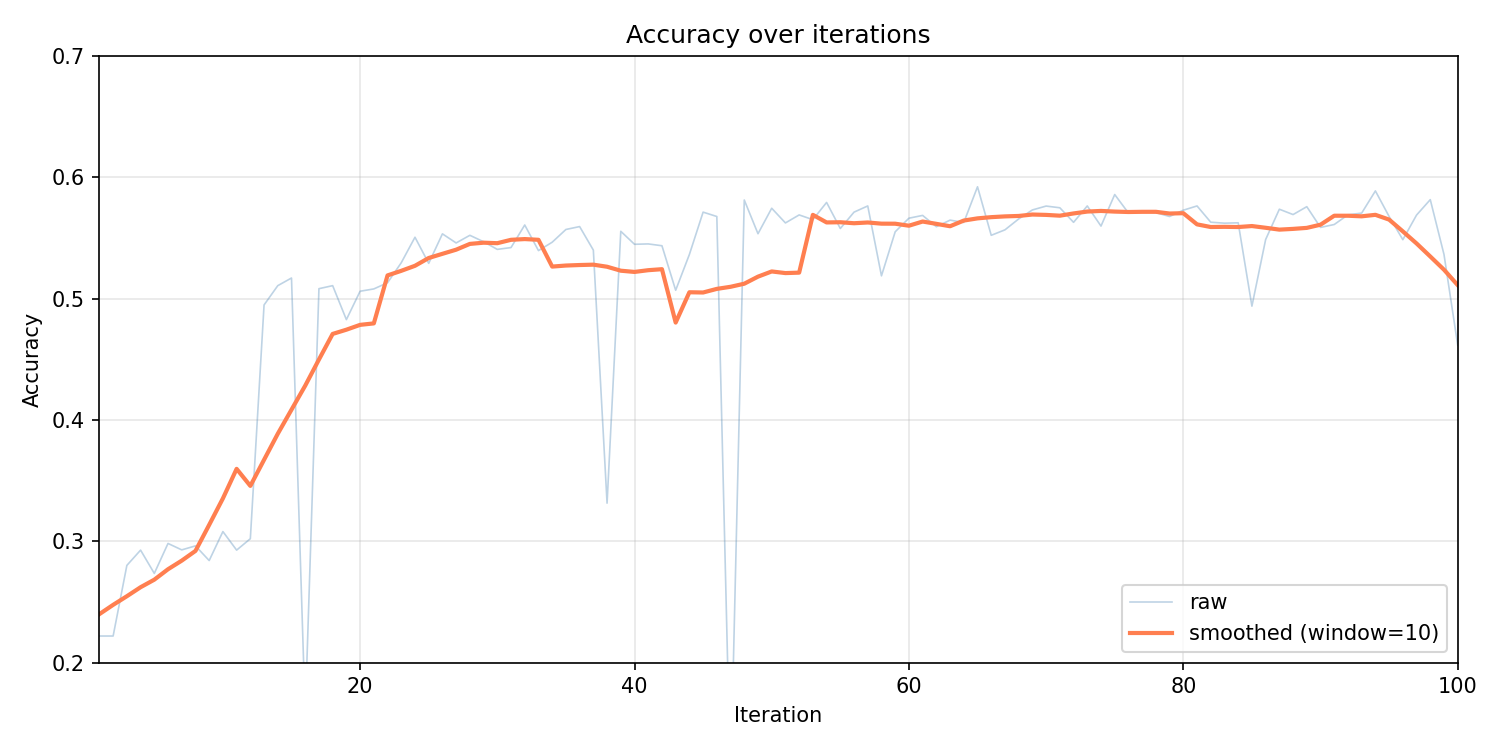
\includegraphics[width=1.00\linewidth]{img/accuracy_curve.png}
		\caption{One-epoch proxy accuracy on CIFAR-10 across 100 successful architecture evaluations. The pipeline exhibits three phases: rapid improvement (${\sim}22\%$ to ${\sim}50\%$), refinement (${\sim}50\%$ to ${\sim}59\%$), and plateau (${\sim}55$--$59\%$). Spearman $\rho = 0.70$ ($p < 10^{-15}$).}
		\label{fig:accuracy}
	\end{figure}
	
	
	\subsection{Failure Analysis}
	
	Of the approximately 1,000 total generation attempts across the experimental run, roughly 60\% failed before reaching the training stage. We categorize failures into three types:
	
	\begin{itemize}
		\item \textbf{Code validation errors} (47.2\%): The generated model fails structural checks---most commonly \texttt{AttributeError} (referencing undefined layers or modules) and tensor shape mismatches between layers.
		\item \textbf{Code extraction errors} (12.7\%): The LLM output cannot be parsed as valid Python, typically due to syntax errors, unclosed string literals, or malformed code blocks.
		\item \textbf{Other runtime errors} ($<$2\%): Errors during training execution, such as device mismatches or batch normalization failures.
	\end{itemize}
	
	The dominant failure mode---\texttt{AttributeError}---occurs when the LLM hallucinates layer names or forgets to define modules referenced in the forward pass. Despite the approximately 40\% overall success rate, the pipeline's resilience (discarding invalid attempts and continuing) ensures that successfully evaluated architectures exhibit consistent improvement across iterations.
	
	
	\section{Discussion}
	\label{sec:discussion}
	
	\paragraph{Effectiveness of iterative refinement.}
	The strong positive correlation ($\rho = 0.70$) across 100 evaluations confirms that historical feedback memory enables systematic architectural improvement. Access to the last $K{=}5$ improvement attempts provides the LLM with sufficient context to identify recurring failure patterns and avoid previously unsuccessful strategies. Notably, the three-phase convergence behavior (rapid improvement, refinement, plateau) mirrors patterns in traditional optimization, suggesting that the LLM-driven search exhibits meaningful optimization dynamics rather than random exploration.
	
	\paragraph{One-epoch proxy as architecture ranking signal.}
	Using one-epoch accuracy as a ranking signal offers a pragmatic trade-off between evaluation cost and informativeness. While the absolute accuracy values (22--59\%) are well below state-of-the-art CIFAR-10 results with full training (exceeding 95\%), prior work on training-free NAS~\cite{Mellor2021,Li2024ZeroShot} has established that cheap proxy metrics can effectively rank architectures. Our one-epoch proxy serves a similar role: it distinguishes between architectures of varying quality at minimal cost, enabling the feedback loop to guide the LLM toward better designs. Retraining the best-discovered architectures with full training schedules could verify whether the one-epoch ranking transfers to converged performance.
	
	\paragraph{Limitations.}
	Our study has several limitations. First, we report a single experimental run with one LLM (Qwen3-4B-Instruct); multi-run experiments and cross-model comparisons would strengthen generalizability. Second, the one-epoch proxy may not perfectly correlate with full-training performance; retraining top architectures to convergence is needed to assess their true potential. Third, the ${\sim}40\%$ code generation success rate indicates that current LLMs still struggle with structurally valid neural network code, suggesting opportunities for improved prompting strategies or constrained decoding. Finally, our evaluation is limited to CIFAR-10; experiments on larger-scale benchmarks and diverse tasks would better demonstrate versatility.
	
	\paragraph{Future work.}
	Promising directions include: (1)~retraining the top-$K$ discovered architectures with full training schedules to verify their converged performance; (2)~comparing across LLMs of varying sizes and families; (3)~integrating zero-shot proxy metrics~\cite{Mellor2021,Li2024ZeroShot} as complementary evaluation signals to further accelerate the search; and (4)~extending to larger datasets (e.g., ImageNet) and tasks beyond image classification.
	
	
	\section{Conclusion}
	\label{sec:conclusion}
	
	We presented an iterative NAS pipeline that leverages a small (4B-parameter) LLM to progressively generate and improve neural network architectures through a closed loop of code generation, evaluation, and prompt refinement with historical feedback memory. Over 100 successful evaluations on CIFAR-10, the pipeline improved one-epoch proxy accuracy from 22.2\% to 59.2\% (Spearman $\rho = 0.70$, $p < 10^{-15}$), demonstrating that iterative feedback with bounded historical memory significantly outperforms single-shot generation. Our results establish that small LLMs can serve as effective architecture search agents when equipped with structured iterative feedback, offering a lightweight and accessible approach to neural architecture search.
	
	{
		\small
		\bibliographystyle{ieeenat_fullname}
		\bibliography{bibmain}
	}
	
\end{document}
